\section{Jalons principaux du projet et lotissement}
\subsection{Jalons du planning EIP Epitech}
Cet ensemble de jalons est commun à tous les groupes, car imposé par le planning EIP.


Une première famille de jalons est formée par les bilans d'architecture AA1 et AA2, respectivement du 20 juin et 1er septembre 2013. Ces jalons devront donc mettre terme aux choix et possibilités au niveau de l'architecture du projet.

Une seconde concerne les bilans techniques, et bilans techniques finaux, répartis de façon régulière de novembre 2013 à janvier 2015. Ils s'axeront avec des jalons propres à notre projet et devront marquer des tournants décisifs, tels que des finalisations de lots.


Enfin, la troisième rassemble les deux soutenances finales, de 4ème année en septembre 2014, et de 5ème en février 2015. Ils représenteront pour leur part des livraisons de versions avancée pour la première, et finale pour la seconde.


\subsection{Jalons propres au projet Onitu}
Ces jalons sont définis au niveau de notre projet et marquent donc des points importants de celui-ci. Ils sont à mettre en parallèle avec l'ensemble précédent, dans le sens où ces derniers représentaient des dates importantes, pour lesquelles ces points devront être atteints.


Tout d'abord, il sera nécessaire de posséder un client minimal de test, pour permettre le développement du serveur, tout en continuant celui du client.


Ensuite, l'obtention d'un serveur fonctionnel, puis d'un serveur complet et fonctionnel marqueront deux étapes très importantes du projet.


Les derniers jalons concernent les clients, et correspondent à la finalisation du fork du client officiel, et de la webUI.


\subsection{Définition du lotissement}
Notre lotissement est formé des différentes parties du projet, à savoir: le fork du client officiel Ubuntu One (ajoutant le choix du serveur à utiliser), la webUI (interface complète de gestion avec partage de fichiers), le serveur (conception et réalisation des API, de la base de données), et les drivers (Donnant accès à des ressources internes comme externes pour le stockage des données).

\newpage

\section{WBS}
\begin{figure}[ht]
    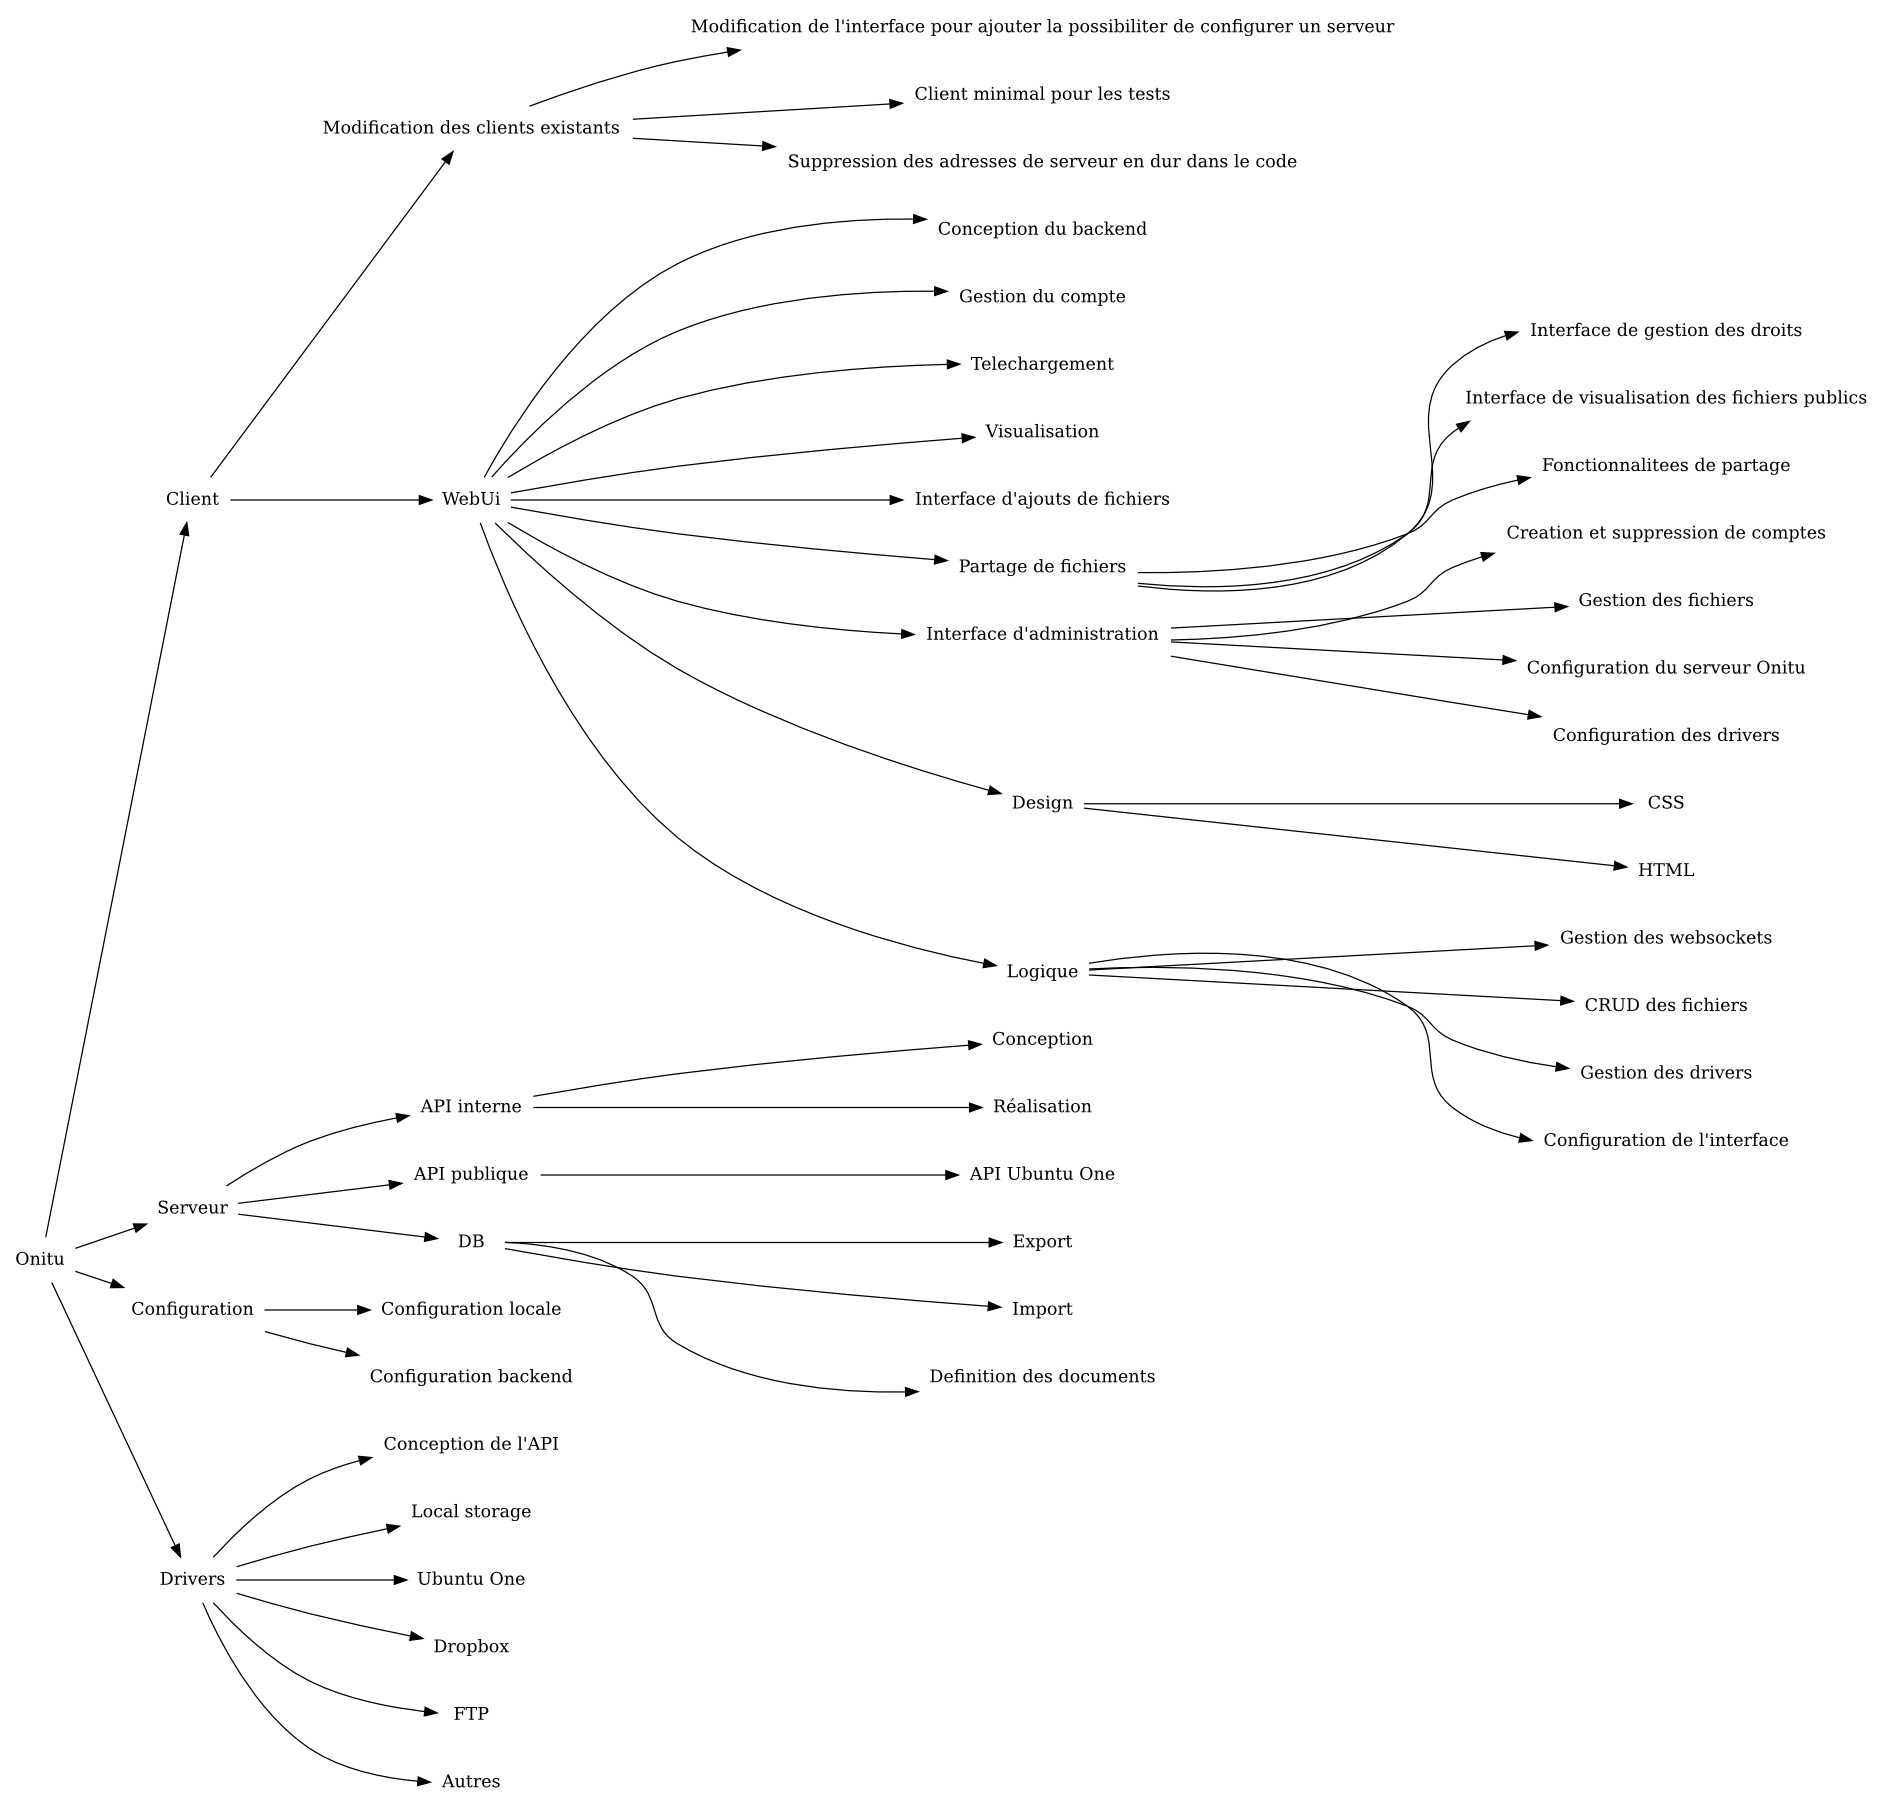
\includegraphics[width=\textwidth,height=\textheight,keepaspectratio]{wbs.png}
    \caption{Work Breakdown Structure}
\end{figure}

\section{Gantt}

\begin{tikzpicture}[y=0.6cm]
  \begin{ganttchart}
    [vgrid,y unit chart=0.5cm, bar height=0.5]{23}
\gantttitle {Gantt Onitu}{23} \\
\gantttitlelist{2013}{8} \gantttitlelist{2014}{12} \gantttitlelist{2015}{3} \\
\gantttitlelist{5,...,12}{1} \gantttitlelist{1,...,12}{1} \gantttitlelist{1, 2, 3}{1}\\
\ganttgroup {LabEIP}{1}{22} \\
\ganttmilestone{Communication}{14}
\ganttmilestone[inline, milestone label inline anchor/.style={left=5pt}]{Plan de promotion exterieure}{14}
\ganttmilestone[inline, milestone label inline anchor/.style={right=5pt}]{Forum eip}{18.5} \\
\ganttmilestone{Bilans}{14.5}
\ganttmilestone[inline, milestone label inline anchor/.style={left=5pt}]{tech final tek4}{14.5}
\ganttmilestone[inline, milestone label inline anchor/.style={left=5pt}]{tech final}{21} \\
\ganttmilestone{Soutenances}{3}
\ganttmilestone[inline, milestone label inline anchor/.style={right=5pt}]{bilan architecture}{3}
\ganttmilestone[inline, milestone label inline anchor/.style={left=5pt}]{finale tek5}{22}
\ganttmilestone[inline, milestone label inline anchor/.style={left=5pt}]{finale tek4}{17} \\
\ganttgroup {Onitu}{1}{21} \\
\ganttgroup {Client}{6}{21} \\
\ganttgroup {Modification clients}{6}{14} \\
\ganttbar {Modification des interfaces }{11}{13}
\ganttbar [inline, bar label inline anchor/.style={left=20pt}]{[Groupe client] 5j/h }{11}{13} \\
\ganttbar {Client minimal pour les tests}{6}{7}
\ganttbar [inline, bar label inline anchor/.style={left=20pt}]{[] j/h }{6}{7} \\
\ganttbar {Suppression des adresses en dur}{13}{14}
\ganttbar [inline, bar label inline anchor/.style={left=20pt}]{[] j/h }{13}{14} \\
\ganttgroup {WebUi}{9}{21} \\
\ganttbar {Conception du backend}{9}{12}
\ganttbar [inline, bar label inline anchor/.style={left=20pt}]{[] j/h }{9}{12} \\
\ganttbar {Gestion du compte}{16}{19}
\ganttbar [inline, bar label inline anchor/.style={left=20pt}]{[] j/h }{16}{19} \\
\ganttbar {Telechargement}{16}{18}
\ganttbar [inline, bar label inline anchor/.style={left=20pt}]{[] j/h }{16}{18} \\
\ganttbar {Visualisation}{21}{21}
\ganttbar [inline, bar label inline anchor/.style={left=20pt}]{[] j/h }{21}{21} \\
\ganttbar {Interface d'ajouts de fichiers}{16}{18}
\ganttbar [inline, bar label inline anchor/.style={left=20pt}]{[] j/h }{16}{18} \\
\ganttgroup {Partage de fichiers}{17}{21} \\
\ganttbar {Gestion des droits}{17}{20}
\ganttbar [inline, bar label inline anchor/.style={left=20pt}]{[] j/h }{17}{20} \\
\ganttbar {Visualisation des fichiers publics}{20}{21}
\ganttbar [inline, bar label inline anchor/.style={left=20pt}]{[] j/h }{20}{21} \\
\ganttbar {Fonctionnalitees de partage}{18}{19}
\ganttbar [inline, bar label inline anchor/.style={left=20pt}]{[] j/h }{18}{19} \\
\ganttgroup {Interface d'administration}{12}{14} \\
\ganttbar {Creation et suppression de comptes}{13}{13}
\ganttbar [inline, bar label inline anchor/.style={left=20pt}]{[] j/h }{13}{13} \\
\ganttbar {Gestion des fichiers}{12}{14}
\ganttbar [inline, bar label inline anchor/.style={left=20pt}]{[] j/h }{12}{14} \\
\ganttbar {Configuration du serveur Onitu}{12}{13}
\ganttbar [inline, bar label inline anchor/.style={left=20pt}]{[] j/h }{12}{13} \\
\ganttbar {Configuration des drivers}{12}{13}
\ganttbar [inline, bar label inline anchor/.style={left=20pt}]{[] j/h }{12}{13} \\
\ganttgroup {Design}{15}{16} \\
\ganttbar {CSS}{15}{16}
\ganttbar [inline, bar label inline anchor/.style={left=20pt}]{[] j/h }{15}{16} \\
\ganttbar {HTML}{15}{16}
\ganttbar [inline, bar label inline anchor/.style={left=20pt}]{[] j/h }{15}{16} \\
\ganttgroup {Logique}{10}{16} \\
\ganttbar {Gestion des websockets}{13}{16}
\ganttbar [inline, bar label inline anchor/.style={left=20pt}]{[] j/h }{13}{16} \\
\ganttbar {CRUD des fichiers}{12}{14}
\ganttbar [inline, bar label inline anchor/.style={left=20pt}]{[] j/h }{12}{14} \\
\ganttbar {Gestion des drivers}{10}{12}
\ganttbar [inline, bar label inline anchor/.style={left=20pt}]{[] j/h }{10}{12} \\
\ganttbar {Configuration de l'interface}{10}{11}
\ganttbar [inline, bar label inline anchor/.style={left=20pt}]{[] j/h }{10}{11} \\
\end{ganttchart}
\end{tikzpicture}

\begin{tikzpicture}[y=0.8cm]
\begin{ganttchart}
    [vgrid,y unit chart=0.7cm, bar height=0.6]{23}
\gantttitle {Gantt Onitu}{23} \\
\gantttitlelist{2013}{8} \gantttitlelist{2014}{12} \gantttitlelist{2015}{3} \\
\gantttitlelist{5,...,12}{1} \gantttitlelist{1,...,12}{1} \gantttitlelist{1, 2, 3}{1}\\
\ganttgroup {LabEIP}{1}{22} \\
\ganttmilestone{Communication}{14}
\ganttmilestone[inline, milestone label inline anchor/.style={left=5pt}]{Plan de promotion exterieure}{14}
\ganttmilestone[inline, milestone label inline anchor/.style={right=5pt}]{Forum eip}{18.5} \\
\ganttmilestone{Bilans}{14.5}
\ganttmilestone[inline, milestone label inline anchor/.style={left=5pt}]{tech final tek4}{14.5}
\ganttmilestone[inline, milestone label inline anchor/.style={left=5pt}]{tech final}{21} \\
\ganttmilestone{Soutenances}{3}
\ganttmilestone[inline, milestone label inline anchor/.style={right=5pt}]{bilan architecture}{3}
\ganttmilestone[inline, milestone label inline anchor/.style={left=5pt}]{finale tek5}{22}
\ganttmilestone[inline, milestone label inline anchor/.style={left=5pt}]{finale tek4}{17} \\
\ganttgroup {Onitu}{1}{21} \\
\ganttgroup {Serveur}{1}{18} \\
\ganttgroup {API interne}{1}{10} \\
\ganttbar {Conception}{1}{8}
\ganttbar [inline, bar label inline anchor/.style={right=20pt}]{[] j/h }{1}{8} \\
\ganttbar {Réalisation}{6}{10}
\ganttbar [inline, bar label inline anchor/.style={right=20pt}]{[] j/h }{6}{10} \\
\ganttgroup {API publique}{6}{10} \\
\ganttbar {API Ubuntu One}{6}{10}
\ganttbar [inline, bar label inline anchor/.style={right=20pt}]{[] j/h }{6}{10} \\
\ganttgroup {DB}{6}{12} \ganttbar {Export}{11}{12} \\
\ganttbar [inline, bar label inline anchor/.style={right=20pt}]{[] j/h }{11}{12} \\
\ganttbar {Import}{11}{12}
\ganttbar [inline, bar label inline anchor/.style={right=20pt}]{[] j/h }{11}{12} \\
\ganttbar {Definition des documents}{6}{7}
\ganttbar [inline, bar label inline anchor/.style={right=20pt}]{[] j/h }{6}{7} \\
\ganttgroup {Configuration}{8}{11} \\
\ganttbar {Configuration locale}{9}{11}
\ganttbar [inline, bar label inline anchor/.style={right=20pt}]{[] j/h }{9}{11} \\
\ganttbar {Configuration backend}{8}{11}
\ganttbar [inline, bar label inline anchor/.style={right=20pt}]{[] j/h }{8}{11} \\
\ganttgroup {Drivers}{1}{18} \\
\ganttbar {Conception de l'API}{1}{7}
\ganttbar [inline, bar label inline anchor/.style={right=20pt}]{[] j/h }{1}{7} \\
\ganttbar {Local storage}{6}{8}
\ganttbar [inline, bar label inline anchor/.style={right=20pt}]{[] j/h }{6}{8} \\
\ganttbar {Ubuntu One}{6}{8}
\ganttbar [inline, bar label inline anchor/.style={right=20pt}]{[] j/h }{6}{8} \\
\ganttbar {Dropbox}{9}{12}
\ganttbar [inline, bar label inline anchor/.style={right=20pt}]{[] j/h }{9}{12} \\
\ganttbar {FTP}{11}{13}
\ganttbar [inline, bar label inline anchor/.style={right=20pt}]{[] j/h }{11}{13} \\
\ganttbar {Autres}{13}{18}
\ganttbar [inline, bar label inline anchor/.style={right=20pt}]{[] j/h }{13}{18} \\
\end{ganttchart}
\end{tikzpicture}
